% Figures for MODELING.md — system block diagram + free-body diagrams.
% Compile:  pdflatex figures.tex   (produces figures.pdf, one figure per page)
\documentclass[11pt]{article}
\usepackage[margin=1in]{geometry}
\usepackage{amsmath}
\usepackage{tikz}
\usetikzlibrary{arrows.meta,positioning,calc,patterns,angles,quotes,decorations.pathmorphing}
\pagestyle{empty}

\tikzset{
  blk/.style={draw,rounded corners,minimum height=9mm,minimum width=20mm,align=center,font=\small},
  sig/.style={-{Stealth[length=2mm]},thick},
  frc/.style={-{Stealth[length=3mm]},very thick},
  gnd/.style={pattern=north east lines,draw},
}

\begin{document}

% ───────────────────────── Fig 1: system block diagram ─────────────────────────
\begin{center}\textbf{Fig.\ 1 — Sim rover as a cascade (which parameter lives in which block)}\end{center}
\begin{center}
\begin{tikzpicture}[node distance=7mm and 12mm]
  \node[blk] (cmd) {\texttt{/cmd\_vel}\\$(v_c,\omega_c)$};
  \node[blk,right=of cmd] (ctrl) {Controller\\$R,\ D$};
  \node[blk,right=of ctrl] (drv) {Wheel drives $\times4$\\$b,\ \tau_{\max}$};
  \node[blk,right=of drv] (con) {Contact\\$\mu_w,\mu_f,C_{rr}$};
  \node[blk,right=of con] (bod) {Chassis\\$m,I_{zz},d_\ell,d_a$};
  \node[blk,right=of bod] (pose) {Pose\\$(x,y,\theta)$};
  \draw[sig] (cmd) -- (ctrl);
  \draw[sig] (ctrl) -- node[above,font=\scriptsize]{$\omega^\*_{L,R}$} (drv);
  \draw[sig] (drv) -- node[above,font=\scriptsize]{$\tau_i$} (con);
  \draw[sig] (con) -- node[above,font=\scriptsize]{$F_{x,i}$} (bod);
  \draw[sig] (bod) -- node[above,font=\scriptsize]{$v,\omega$} (pose);
  \node[font=\scriptsize,below=2mm of ctrl,align=center]{eq.\,(4.1)};
  \node[font=\scriptsize,below=2mm of drv,align=center]{eq.\,(2.1)};
  \node[font=\scriptsize,below=2mm of con,align=center]{eq.\,(3.1)--(3.3)};
  \node[font=\scriptsize,below=2mm of bod,align=center]{eq.\,(5.1)--(5.2)};
  \draw[sig,dashed] (pose.south) .. controls +(0,-1) and +(0,-1) .. node[below,font=\scriptsize]{camera / \texttt{/odom} (measured)}(cmd.south);
\end{tikzpicture}
\end{center}
\vspace{4mm}
\hrule

% ───────────────────────── Fig 2: drivetrain FBD + servo block ──────────────────
\begin{center}\textbf{Fig.\ 2 — Actuator: motor $\to$ axle $\to$ wheel (eq.\ 2.1, 2.4)}\end{center}
\begin{center}
\begin{tikzpicture}
  % motor + gearbox + wheel
  \node[draw,minimum width=14mm,minimum height=10mm] (mot) at (0,0) {Motor};
  \node[draw,minimum width=10mm,minimum height=10mm,right=4mm of mot] (gb) {Gear $G$};
  \draw[very thick] (gb.east) -- ++(1.2,0) node[midway,above,font=\scriptsize]{axle};
  \draw[fill=gray!15] ($(gb.east)+(2.2,0)$) circle (1cm);
  \node at ($(gb.east)+(2.2,0)$) {wheel $r$};
  % applied torque
  \draw[frc] ($(gb.east)+(2.2,1.2)$) arc (90:0:1.2) node[right,font=\small]{$\tau_i$};
  % electrical label
  \node[font=\scriptsize,below=1mm of mot,align=center]{$L_a\dot i{+}R_a i{=}V{-}K_e\omega_m$\\$J_m\dot\omega_m{=}K_t i{-}\tau_L/G$};
  % servo control block
  \node[blk,right=28mm of gb,yshift=0mm] (sum) {$b(\omega^\*{-}\omega)$};
  \node[blk,right=6mm of sum] (clip) {clamp\\$\pm\tau_{\max}$};
  \draw[sig] (sum) -- (clip);
  \draw[sig] (clip.east) -- ++(1,0) node[right,font=\small]{$\tau_i$};
  \node[font=\scriptsize,above=1mm of sum,align=center]{stiff velocity servo};
  \node[font=\scriptsize,below=5mm of clip,align=center,text width=5cm]{authored $b{=}10^4$ (near-ideal speed source) $\Rightarrow$ ramp is set by $\tau_{\max}$, eq.\,(2.3)};
\end{tikzpicture}
\end{center}
\vspace{4mm}
\hrule

% ───────────────────────── Fig 3: wheel–ground contact FBD ──────────────────────
\begin{center}\textbf{Fig.\ 3 — Wheel against the ground: friction cone \& slip (eq.\ 3.1--3.4)}\end{center}
\begin{center}
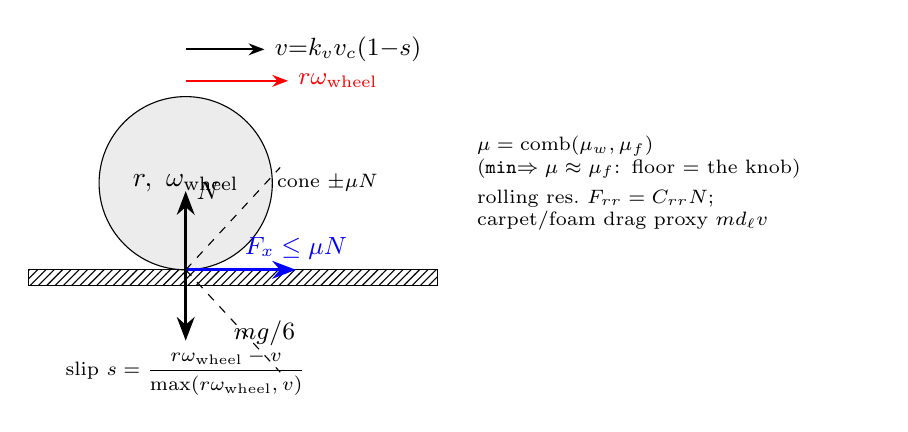
\begin{tikzpicture}
  \fill[gray!15] (-3,0) circle (1.1cm);
  \draw (-3,0) circle (1.1cm);
  \node at (-3,0) {$r,\ \omega_{\text{wheel}}$};
  \draw[gnd] (-5,-1.1) rectangle (0.2,-1.3);           % ground
  \coordinate (C) at (-3,-1.1);                          % contact point
  \draw[frc] (C) -- ++(0,1.0) node[right,font=\small]{$N$};
  \draw[frc] (C) -- ++(0,-0.9) node[right,font=\small]{};
  \node[font=\small] at (-2.0,-1.9) {$mg/6$};
  \draw[frc,blue] (C) -- ++(1.4,0) node[above,font=\small]{$F_x\le\mu N$};
  % friction cone
  \draw[dashed] (C) -- ++(1.2,1.3);
  \draw[dashed] (C) -- ++(1.2,-1.3);
  \node[font=\scriptsize] at (-1.2,0.0) {cone $\pm\mu N$};
  % velocities
  \draw[sig,red] (-3,1.3) -- ++(1.3,0) node[right,font=\small]{$r\omega_{\text{wheel}}$};
  \draw[sig] (-3,1.7) -- ++(1.0,0) node[right,font=\small]{$v{=}k_v v_c(1{-}s)$};
  \node[font=\scriptsize,align=center] at (-3,-2.4){slip $s=\dfrac{r\omega_{\text{wheel}}-v}{\max(r\omega_{\text{wheel}},v)}$};
  \node[font=\scriptsize,align=left,text width=5cm] at (3.2,0){$\mu=\mathrm{comb}(\mu_w,\mu_f)$\\ (\texttt{min}$\Rightarrow\mu\approx\mu_f$: floor = the knob)\\[1mm] rolling res.\ $F_{rr}=C_{rr}N$;\\ carpet/foam drag proxy $m d_\ell v$};
\end{tikzpicture}
\end{center}
\vspace{4mm}
\hrule

% ───────────────────────── Fig 4: skid-steer ICR top view ───────────────────────
\begin{center}\textbf{Fig.\ 4 — Skid-steer kinematics (top view): effective track \& under-rotation (eq.\ 4.1--4.3)}\end{center}
\begin{center}
\begin{tikzpicture}
  \draw[thick] (-1,-1.5) rectangle (1,1.5);              % chassis (top view)
  \node at (0,0) {\small body};
  % wheels
  \foreach \y in {-1.1,0,1.1}{
    \draw[fill=gray!25] (-1.25,\y-0.18) rectangle (-0.95,\y+0.18);
    \draw[fill=gray!25] ( 0.95,\y-0.18) rectangle ( 1.25,\y+0.18);
  }
  % wheel velocities
  \draw[sig,red] (-1.1,1.1) -- ++(0,-0.8) node[left,font=\scriptsize]{$-\omega_L^\*$};
  \draw[sig,blue] (1.1,1.1) -- ++(0,0.8) node[right,font=\scriptsize]{$+\omega_R^\*$};
  % ICR
  \fill (3.2,0) circle (1.2pt) node[above,font=\scriptsize]{ICR};
  \draw[dashed] (0,0) -- (3.2,0) node[midway,above,font=\scriptsize]{$R_{\text{arc}}$};
  \draw[{Stealth[length=2mm]}] (0.4,0.6) arc (60:120:0.8) node[above,font=\small]{$\omega$};
  % B and D
  \draw[<->] (-1.1,-1.75) -- (1.1,-1.75) node[midway,below,font=\scriptsize]{physical track $B$};
  \draw[<->] (-1.6,-2.2) -- (1.6,-2.2) node[midway,below,font=\scriptsize]{effective $D=\chi B$ (calibrated)};
  \node[font=\scriptsize,align=left,text width=5.2cm] at (4.6,-0.6){$\omega=\dfrac{k_v D}{\chi B}\,\omega_c$\\[1mm]$\chi\!\ge\!1$ grows with grip $\Rightarrow$ raise $D$ on higher-$\mu$ floors (fit $D$ after $\mu$).};
\end{tikzpicture}
\end{center}
\vspace{4mm}
\hrule

% ───────────────────────── Fig 5: chassis planar FBD ────────────────────────────
\begin{center}\textbf{Fig.\ 5 — Chassis planar free-body diagram (eq.\ 5.1--5.2)}\end{center}
\begin{center}
\begin{tikzpicture}
  \draw[thick,fill=gray!8] (-1.4,-0.9) rectangle (1.4,0.9);
  \node at (0,0) {\small $m,\ I_{zz}$};
  \draw[frc,blue] (1.4,0.4) -- ++(1.6,0) node[right,font=\small]{$F_{\text{drive}}\le \min(\mu N, n_d\tau_{\max}/r)$};
  \draw[frc,red] (-1.4,-0.4) -- ++(-1.4,0) node[left,font=\small]{$C_{rr}mg+m d_\ell v$};
  \draw[{Stealth[length=2mm]}] (0.6,0.0) arc (-30:210:0.5);
  \node[font=\small] at (0,1.25) {$M_{\text{drive}}-M_{\text{scrub}}(\mu)-I_{zz}d_a\omega$};
  \node[font=\scriptsize,align=left,text width=11cm] at (0,-1.9){
    $m_{\mathrm{eff}}\dot v=F_{\text{drive}}-C_{rr}mg-m d_\ell v$ \qquad
    $I_{zz,\mathrm{eff}}\dot\omega=M_{\text{drive}}-M_{\text{scrub}}-I_{zz,\mathrm{eff}}d_a\omega$\\
    coast ($v_c{=}0$): brake $=\min(n_d b\,v/r^2,\ n_d\tau_{\max}/r)$ $\Rightarrow$ $d_{\text{coast}}\approx v_0^2/2a_{\text{brake}}$ (eq.\,5.6)};
\end{tikzpicture}
\end{center}

\end{document}
